\chapter{Results}\label{chapter:5}

%\section{Experiment setup}

We use~\cite{terada} for sensor specification. The sensors are ZigBee temperature sensors, collecting data at one reading per second. In~\cite{terada}, the authors have used 12~bits for one temperature reading. Therefore, our $SSR$ (sensor data sampling rate) is expected to be 1.25 byte/second. The $SDT$ (sensor data throughput) is taken to be 13.4 kbps~\cite{zigbee}. The MULEs' speed is taken to be 10m/s~\cite{muleSpeed}. The sensor positions are chosen randomly in a field of 1000m~$\times$~1000m, and the sensor range is 50m. Note that Zigbee sensor ranges can lie between 10m to 100m.

\section{Simulation results}
We now present simulation results of our heuristic applied on the following 6 cases:
\begin{itemize}
\item Field size: All Cases: 1000m $\times$ 1000m
\item Sensor Range: All cases: 50 m
\item Number of sensors: Case 1: 50, Case 2: 60, Case 3: 70, Case 4: 80, Case 5: 90, Case 6: 100
\end{itemize}

For each of the above cases we generate 6 random distributions of the sensors, and apply our heuristic on each of them with latency bound of 100 seconds, increasing in steps of 100s until only one MULE is adequate to cover the whole field. The graph "Number of MULEs required vs Required latency bound" for a case is the plot of required latency bound in X-axis, versus, average number of MULEs required to satisfy the latency bound in that case across its 6 random distributions, in Y-axis. The graph "Average latency achieved vs Number of MULEs employed" for a case is the plot of number of MULEs employed in the case in X-axis, versus, the average latency achieved by these many MULEs in this case, across the 6 random distributions.

Each of the following subsections contain results for the respective cases.

As we can see from the "Number of MULEs required vs Required latency bound" graphs of each case, the decrease in number of MULEs required to fulfill the required latency bound, is not uniform with respect to the increase in the latency bound. For instance, in 70 sensors case, for an increase of latency bound from 100 seconds to 290 seconds decreases the num,ber of MULEs required from 13 to 6. However, for further drop in number of MULEs from 6 to 1, the increase in latency bound is from 290 seconds to 1140 seconds. Similarly, from the "Average latency achieved vs Number of MULEs employed" graphs of each case, we can observe that the decrease in the affordable latency bound is not uniform with respect to the increase in the number of MULEs employed. E.g in 70 sensors case, increasing the number of MULEs from 1 to 8 causes the affordable latency to drop from 1100 seconds to 202 seconds. But, a further increase of 7 MULEs decreases the latency only to 100 seconds. Therefore, we can conclude that the relation between latency bound and the number of MULEs required is not linear, and after a certain number of MULEs employed, additional MULEs do not achieve significant latency decrease. Let us call this number of MULEs a "flat point" for convinience of reference. Also, let the number of MULEs to achieve latency of 100 seconds in a case be called its "max point". The existence of flat points should be apparent from the table below. Let $\delta f$ be decrease in latency from 1 MULE to flat point and $\delta m$ be decrease in latency from flat point to max point in the following table.

\begin{center}
 \begin{tabular}{||c c c c c||} 
 \hline
 Number of sensors & max point & flat point & $\delta f$ & $\delta m$ \\  
 \hline\hline
 50 & 15 & 8 & 790 s & 120 s\\ 
 \hline
 60 & 14 & 9 & 872 s & 68 s\\
 \hline
 70 & 15 & 8 & 897 s & 102 s\\
 \hline
 80 & 15 & 9 & 1042 s & 106 s\\
 \hline
 90 & 17 & 9 & 1076 s & 144 s\\
 \hline
 100 & 18 & 11 & 1155 s & 113 s\\
 \hline
\end{tabular}
\end{center}

\pagebreak

\subsection{50 sensors}
\begin{figure}[H]
\includegraphics[width=15cm]{50/res_avg.png}
\caption{Number of MULEs required vs Required latency bound for 50 sensors}
\end{figure}
\begin{figure}[H]
\includegraphics[width=15cm]{50/res_lat.png}
\caption{Average latency achieved vs Number of MULEs employed for 50 sensors}
\end{figure}
\subsection{60 sensors}
\begin{figure}[H]
\includegraphics[width=15cm]{60/res_avg.png}
\caption{Number of MULEs required vs Required latency bound for 60 sensors}
\end{figure}
\begin{figure}[H]
\includegraphics[width=15cm]{60/res_lat.png}
\caption{Average latency achieved vs Number of MULEs employed for 60 sensors}
\end{figure}

\subsection{70 sensors}
\begin{figure}[H]
\includegraphics[width=15cm]{70/res_avg.png}
\caption{Number of MULEs required vs Required latency bound for 70 sensors}
\end{figure}
\begin{figure}[H]
\includegraphics[width=15cm]{70/res_lat.png}
\caption{Average latency achieved vs Number of MULEs employed for 70 sensors}
\end{figure}

\subsection{80 sensors}
\begin{figure}[H]
\includegraphics[width=15cm]{80/res_avg.png}
\caption{Number of MULEs required vs Required latency bound for 80 sensors}
\end{figure}
\begin{figure}[H]
\includegraphics[width=15cm]{80/res_lat.png}
\caption{Average latency achieved vs Number of MULEs employed for 80 sensors}
\end{figure}

\subsection{90 sensors}
\begin{figure}[H]
\includegraphics[width=15cm]{90/res_avg.png}
\caption{Number of MULEs required vs Required latency bound for 90 sensors}
\end{figure}
\begin{figure}[H]
\includegraphics[width=15cm]{90/res_lat.png}
\caption{Average latency achieved vs Number of MULEs employed for 90 sensors}
\end{figure}

\subsection{100 sensors}
\begin{figure}[H]
\includegraphics[width=15cm]{100/res_avg.png}
\caption{Number of MULEs required vs Required latency bound for 100 sensors}
\end{figure}
\begin{figure}[H]
\includegraphics[width=15cm]{100/res_lat.png}
\caption{Average latency achieved vs Number of MULEs employed for 100 sensors}
\end{figure}
